\documentclass[a4paper]{article}
\usepackage{a4wide}
\usepackage{graphicx}

\begin{document}

\begin{center}
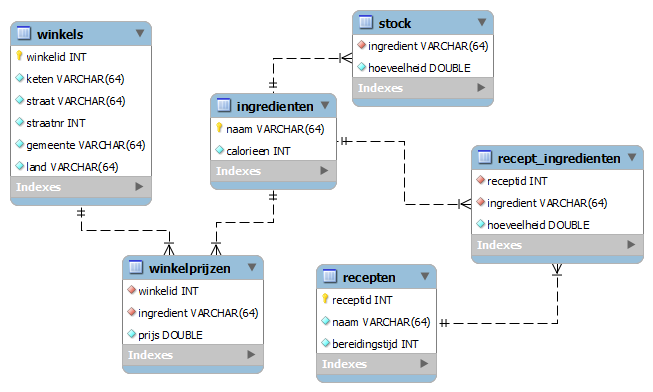
\includegraphics[width=\textwidth]{schema.png}
\end{center}

\begin{itemize}
  \item (\textsc{select}) Voor elk recept is er een bepaalde hoeveelheid van bepaalde ingredi\"enten nodig.
        Elk ingredi\"ent bevat een zeker aantal calorie\"en.
        Reken per recept het totaal aantal calorie\"en uit (rekening houdend
        met welk ingredi\"ent, de hoeveelheid, en het aantal calorie\"en) en
        sorteer ze van calorierijkst tot caloriearmst.
        \begin{center}
          \begin{tabular}{c|c}
            {\bf receptnaam} & {\bf totaal\_cal}
          \end{tabular}
        \end{center}
  \item (\textsc{select})Zoek voor het recept voor chocoladecake
        op welke winkel voor elk ingredi\"ent apart het goedkoopst is.
        De uitvoer moet per ingredi\"ent dat nodig is voor
        de bereiding van een chocoladecake aangeven waar dit
        ingredi\"ent het minst kost. De uitvoer moet eveneens deze laagste prijs weergeven.
        \begin{center}
          \begin{tabular}{c|c|c|c|c}
            {\bf ingredient} & {\bf keten} & {\bf gemeente} & {\bf straat} & {\bf prijs}
          \end{tabular}
        \end{center}
  \item (\textsc{select})De stock bevat de ingredi\"enten die we op voorraad hebben.
        Gegeven een recept zal het nodig zijn om bepaalde ingredi\"enten
        te moeten gaan bijkopen. Zoek voor elk recept per winkel op hoeveel
        het kost om de ontbrekende ingredi\"enten aan te kopen.
        Je mag ervan uitgaan dat winkels elk ingredi\"ent aanbieden,
        maar niet dat de stock een rij bevat voor elk ingredi\"ent.
        We zijn enkel ge\"interesseerd in gevallen waar de totale
        kost kleiner dan of gelijk is aan 3. Sorteer op stijgende kost.
        \begin{center}
          \begin{tabular}{c|c|c|c|c}
            {\bf recept} & {\bf keten} & {\bf gemeente} & {\bf straat} & {\bf kost}
          \end{tabular}
        \end{center}
  \item (\textsc{create table})Maak een extra tabel voor coupons. Een coupon geeft een bepaalde korting
        op een bepaald ingredi\"ent in een bepaalde winkel. Een coupon is geldig
        tot een bepaalde datum. Van elk coupon houdt men bij wanneer men
        het gebruikt heeft (of {\tt NULL} indien nog ongebruikt).
        Een korting wordt bijgehouden als een factor, bv.\ 0.9 voor 10\% korting.
        We willen afdwingen dat de korting een geldige waarde heeft, m.a.w.\ tussen
        0 (exclusief) en 1 (exclusief) ligt.
  \item (\textsc{delete}) De Free Record Shop sluit. Hoewel ze van teleurstellend weinig nut waren
        voor ons kookwerk (zal vermoedelijk ook wel een grote rol gespeeld hebben bij het faillsement ervan)
        stonden hun gegevens in onze database. We willen deze gegevens eruit verwijderen.
        Geef de nodige {\tt DELETE} opdrachten.
  \item (\textsc{update}) We hebben zojuist een heerlijke cr\`eme br\^ul\'ee gemaakt. Hiervoor
        hebben we bepaalde hoe\-veel\-heden ingredi\"enten moeten gebruiken.
        Schrijf een {\tt UPDATE} opdracht die de stock aanpast.
        Ga ervan uit dat de stock van elk ingredi\"ent voldoende op voorraad had.
\end{itemize}



\end{document}
